%\documentclass[twocolumn]{aastex62}
%\documentclass[onecolumn]{aastex62}
\documentclass[modern]{aastex62}

\shorttitle{LSST Community Brokers}
\shortauthors{Guy, Bellm, Graham}

\usepackage{collect}
\usepackage[colorinlistoftodos]{todonotes}

\graphicspath{{./}{./figures/}}

% Environment for recommendations
\providecommand{\secref}[1]{\hyperref[#1]{Section~\ref{#1}}}
\providecommand{\appref}[1]{Appendix~\ref{#1}}
\providecommand{\tabref}[1]{Table~\ref{#1}}
\providecommand{\figref}[1]{Figure~\ref{#1}}
\providecommand{\eqnref}[1]{Eq.~\ref{#1}}
\providecommand{\recref}[1]{\hyperref[#1]{REC-\ref{#1}}}

%Counter for recommendations
\newcounter{reccount} 
\newenvironment{recenv}[1]
    { % empty more or less but we need it so we can refer to it.
    \refstepcounter{reccount}  %increment the counter for each recomendation
    #1
    }

% Recommendations collection
\definecollection{nrecommendations}
%chapter, audience, term, 
%label (rec:label for references), title, full text
\newcommand{\nrec}[3]{ 
	\begin{recenv}
	\vspace{5pt}
	\noindent \textbf{REC-\thereccount~#2}.     
	%\textbf{Area:} #1.  \textbf{Audience:} #2. \textbf {Term:} #3
	\newline \label{rec:#1}\noindent \textit{#3}
	\vspace{5pt}
	\end{recenv}
    % collecting  for output :
    \begin{collect}{nrecommendations}{}{}
        \noindent \textbf{REC-\ref{rec:#1}~#2}.
	%\newline \textbf{Area:} #1.  \textbf{Audience:} #2. \textbf {Term:} #3
        \newline \textit{#3}.
        \newline See page \pageref{rec:#1}. \vspace{10pt}
     \end{collect}
\typeout{REC-\thereccount: #1: #2: #3 :END}
}

% Use these macros for commenting
\newcommand{\ECB}[2][]{\todo[color=blue!30, #1]{EB: #2}}
\newcommand{\MLG}[2][]{\todo[color=red!30, #1]{MLG: #2}}
\newcommand{\LPG}[2][]{\todo[color=cyan!30, #1]{LPG: #2}}

%\newcommand{\docRef}{LSST-Community-Broker-Workshop}
%\newcommand{\docUpstreamLocation}{\url{https://github.com/lsst-dmsst/LSST-Community-Broker-Workshop}}

\begin{document}
\correspondingauthor{Leanne~P.~Guy}
\email{leanne.guy@lsst.org}

\author[0000-0003-0800-8755]{Leanne~P.~Guy}
\affiliation{LSST Project Office, 950 N.\ Cherry Ave., Tucson,  {AZ}  85719,  {USA}}

\author[0000-0001-8018-5348]{Eric C. Bellm}
\affiliation{University of Washington, Dept.\ of Astronomy, Box 351580, Seattle,  {WA} 98195,  {USA}}

\author[0000-0002-9154-3136]{Melissa~L.~Graham}
\affiliation{University of Washington, Dept.\ of Astronomy, Box 351580, Seattle,  {WA} 98195,  {USA}}

\author[0000-0003-1953-8727]{Federica~B.~Bianco}
\affiliation{{Department of Physics and Astronomy, University of Delaware, Newark,  {DE}, 19716,  {USA}
2}}
\affiliation{{Joseph R. Biden, Jr. School of Public Policy and Administration, University of Delaware, Newark,  {DE}, 19716,  {USA}
2}}
\affiliation{{Data Science Institute, University of Delaware, Newark,  {DE}, 19716,  {USA}
2}}
\affiliation{Center for Urban Science \& Progress, New York University, Brooklyn,  {NY} 11021,  {USA}}

\author{Josh~S.~Bloom}
\affiliation{Astronomy Department,  University of California, 601 Campbell Hall, Berkeley,  {CA} 94720, USA}

\author[0000-0002-8622-4237]{Robert~Blum}
\affiliation{LSST Project Office, 950 N.\ Cherry Ave., Tucson,  {AZ}  85719,  {USA}}

\author[0000-0001-5250-2633]{\v{Z}eljko~Ivezi\'{c}}
\affiliation{University of Washington, Dept.\ of Astronomy, Box 351580, Seattle,  {WA} 98195,  {USA}}

\author[0000-0001-6279-0552]{Rachel~A.~Street}
\affiliation{Las Cumbres Observatory, 6740 Cortona Dr., Suite 102, Santa Barbara,  {CA} 93117, USA}
\date{\today}
\title{Transient Alert Brokers in the LSST Era.}


% Leanne to Ensure that the community broker workshop paper includes a statement about the number of brokers we can support and the technical implications 

\begin{abstract}
Beginning late 2022, the Vera C. Rubin Observatory Legacy Survey of Space and Time ( LSST), will produce a nightly stream of ten million public alerts that will disseminate new information about  transient  , variable, and moving objects within 60 seconds.  A number of \emph{Community Brokers} will be selected to receive the full  LSST  alert stream, adding additional scientific value, and providing science users the ability to identify targets of interest and trigger follow-up observations.  In June 2019, the  LSST  project hosted a workshop on \emph{Community Brokers} in Seattle,  WA,  USA. The overarching goal of the workshop was to bring together Rubin Observatory Project personnel, representatives of the  LSST  Science Collaborations, proposers of community brokers and follow-up facilities to develop a vision of an integrated global ecosystem for  transient   science with the  LSST  alert stream. Topics of discussion included, scientific use cases and expectations for the  LSST  Prompt data products,  LSST -broker interfaces, architecture and technology choices, the broker selection process, policy issues, and development progress and lessons learnt from precursor surveys. This paper provides a summary of that workshop and a road-map towards a building a global integrated ecosystem for time-domain science in the  LSST era.

%This document was co-authored during the workshop and edited in months following. It captures the discussions and highlights many ideas that came out of the workshop. 
\end{abstract}




\keywords{LSST, Astronomy, Astrophysics, Algorithms, Brokers, Community Brokers,  {Data Management}, Alerts, Computing,  {HTC}, Networking, Machine Learning, Cloud}

% Only needed while this is a work in progress. Remove for circulation. 
\listoftodos
\clearpage

% Leanne 
\section{Introduction (Leanne)} \label{sec:intro}

{\it Section Status: draft in progress. 
To Do: 
Introduction to transient science with LSST and the challenges posed.  
Brief outline of the LSST strategy - point to section \ref{sec:alertproduction}
Introduce the concept of Community Event Brokers.   
Describe the goals and format of the meeting including the unconference sessions. }

Following the January 2019 'Call for Letters of Intent for Community Alert Brokers'  
\citep{LDM-612}
the LSST Project hosted a workshop with the goal of bringing together representatives of all 

The workshop addressed several topics: 
\begin{itemize}
    \item Science Drivers (section \ref{sec:science}) --- what are the science drivers for Brokers?
    \item Broker Architecture and Technology (section \ref{sec:archandtech}) --- what technology will underpin Broker services 
    \item Algorithms \ref{sec:algorithms}) ---  what kinds of user algorithms do Brokers need to support 
    \item Follow-up infrastructure \ref{sec:followup}) --- how do Brokers interface to follow-up services 
    \item User-facing services \ref{sec:interfaces}) --- how will the scientific community interact with brokers 
\end{itemize}

This paper summarizes the presentations and discussions of the workshop. It highlights many ideas and recommendations that came out of the workshop. The workshop presentations are available at $<someurl>$ and we refer to them throughout this paper.


To address these challenges, we make the following recommendations
% A registry of brokers should be used to facilitate communications such as those
% outlined in ticket:
% DM-20561 Updates for communications with broker proposers (from CBW FAQ)

\nrec{brokerregistry}
{Agency, Technologist}
{Long}
{cbra}
{Investigate how to facilitate setting up a registry of Brokers}
{In order to enable science users to interact with and learn more about brokers and their progress, it was proposed in an Unconference session that some kind of public registry of brokers be created.}
% \newpage
\section{Recommendations} \label{recommendations}

Table \ref{tab:recomendations} provides a high level summary of the recommendations that emerged from this workshop. The labels are linked to the full recommendation in the relevant section of the document.  {\emph Area} describes the work are that the recommendation is targeted at and {\emph Term} the time scale on which the recommendation will be addressed. 
% Note that this table should be auto-generated from the recommendations in the document - need to get the script (this system is taken from a paper of Wil's

%\tiny 
\begin{longtable} {p{0.68\textwidth}  p{0.13\textwidth}  p{0.09\textwidth} }
\hline 
\textbf{Recommendation} &\textbf{Area }& \textbf{Term} \\\hline
% \hyperref[rec:ppdbincloud]{{\textbf REC-1} Rec } & Science & Medium  \\\hline
% \hyperref[rec:5]{{\textbf \tiny REC-5} Rec } & Analysis & Medium    \\\hline
\caption{Workshop Recommendations. \label{tab:recomendations}}
\end{longtable} 
%\normalsize
% \clearpage











% Summary of the workshop session: 
% Science Goals Requiring Community Brokers and related unconference sessions. 

\section{Science Drivers (Melissa)} \label{sec:science}

\LPG[inline]{It would be good to see a table of the timescale demanded for access to alerts by all science cases, similar to what Ashley presented for TVSSC, but for all science goals }

\noindent
{\it Section Status: draft in progress. \\
To Do: \\
Section could be shortened by gathering all the "broker needs" and "problems forseen" from each subsection into a single collated subsection (\S~\ref{ssec:sci_sum}). MLG can do this later. \\ 
Invite the original presenters to review text and be coauthors.\\
Include any other science drivers from the other talks and unconferences.\\ Ensure this section is adequately answering the questions: \\
 - Which science drivers need community brokers and follow-up? \\
 - Which science drivers need the LSST prompt data products (60s and 24h latency)?  \\
 - Which science cases require new approaches? \\
 - What do the LSST science collaborations want to see from community brokers? \\

\LPG[inline] {Suggest to add in a discussion of some of the scientific challenges for LSST alerts; Contrast the luxury of Catalina, which is able to optimize to one science goal to the challenges of LSST, which must accommodate a multitude of science goals}
}

\medskip
This section summarizes the invited presentations from each of the LSST Science Collaborations (SC), which addressed the science drivers that rely on working with the LSST alert stream and/or prompt data products. One of the goals of this session was to ensure that broker developers are informed of the variety of science goals for LSST Prompt products, so that they can develop systems that respond to the science needs. A full overview of LSST science drivers are detailed in the LSST overview paper \cite{2019ApJ...873..111I} ({\bf cite also the science book}).



\subsection{Transients and Variable Stars}\label{ssec:sci_tvs}
% Rep: Ashley Villar
% Material sourced from:
% LSST CBW Participants Drive > Presentations - Wednesday Afternoon > Slides for SC Rep Talks at LSST CBW (TVS)
% LSSTBrokerWorkshop19 > SOC's Notes (private)

The Transients and Variable Stars (TVS) Science Collaboration is focused on studies of intrinsically variable events (periodic and aperiodic), explosive and eruptive transients, as well as extrinsic variables and transients (e.g., eclipsing binaries, microlensing). Science goals include both improving the physical understanding of these systems (e.g., stellar evolution, high-energy astrophysics) and using these objects as distance markers and probes of their environment (e.g., mapping the Milky Way, characterizing the intracluster medium, and dark energy cosmology). The objects which fall under the TVS umbrella span a wide range of timescales and energy outputs, and their studies frequently involve multi-messenger (e.g., neutrinos, gravitational waves) and/or multi-wavelength observations that span the electromagnetic spectrum. 

Some of these TVS science goals require the alerts (and brokers) in order to categorize objects and identify those which need rapid follow-up (e.g., spectroscopy, multi-band photometry) to provide the definitive classification and/or key astrophysical evidence. For example, finding young supernovae within hours of explosion when the optical and near-ultraviolet spectrum exhibit the short-lasting signatures of shock breakout (which can constrain the radius of the progenitor star; {\bf reference}), identifying a $\lesssim$day-long exoplanet feature in a microlensing event, or discovering optical counterparts to gravitational wave events. 

Other TVS science goals which need follow-up on longer time scales (days to weeks) could technically use the Prompt products database (PPDB; {\bf reference paper section}) instead of alerts, but may use the alerts and brokers system infrastructure for classification anyway. For example, identifying supernovae that are nearing peak brightness in order to make the most efficient use of spectroscopic classification resources, or determining when an eclipsing binary has passed a quality threshold (e.g., orbital parameter errors have decreased below a limit) to warrant follow-up. In a survey of the TVS members' needs for alerts and brokers ({\bf how to reference Rachel's report?}), responses to a question about access to difference-image sources were about evenly divided between ``same-night" and ``three days or longer". Respondents were also about equally divided between wanting alerts delivered by VOEvent stream and API subscriber, (more immediate use) or by an online page or email, corresponding to desires for more immediate use and a longer latency, respectively.

Given the diversity of TVS use-cases for an LSST alert broker, there is also a diversity of needed features. Simple filtering -- applying limits on the alert packet contents -- is insufficient for many of the TVS science goals mentioned above, which require several value-added processes. In particular, associating same-night alerts for a new source is necessary to provide a color\footnote{Recall that alerts are issued for sources detected in a single difference-image, and if a source is new and not yet in the PPDB, none of its alerts during its first night of detection will contain association information.}, light-curve fits to and/or feature extraction from the historical data in the alert packet are necessary for categorization, and cross-matching with external catalogs and/or a robust evaluation of host galaxy offset\footnote{The identification of a host galaxy is not always simply the nearest static-sky source, but requires a probabilistic assessment of the offset in effective radii and other galaxy attributes.} are needed for additional contextual information in prioritizing follow-up. The TVS has also identified the science-driven need to characterize the selection biases of brokering systems, which may entail giving users the ability to generate and process simulated events, and the need to broker (or re-broker) alerts from past events (e.g., when an algorithm is updated). 

Triggering follow-up is at the core of TVS's alert-based science goals, and for that, broker systems which facilitate the activation of Target of Opportunity observations are needed -- whether it be by notifying a human, automatically submitting packets to queue-scheduled facilities, or directly scheduling observations with robotic telescopes. Some or all of this triggering process might not happen within the broker, but instead within Target Observation Managers ({\bf reference section of this paper}) to which brokers connect -- and thus interfacing with TOMs is another science-driven need from the TVS perspective.

{\bf Challenges Faced --} First, it is acknowledged that some of the science-driven broker needs, such as feature extraction and processing simulated streams, will require considerable computational resources. Second, obtaining robust categorizations for objects with sparsely sampled light-curves, especially during the hours and days following the start of a photometric event, remains an open challenge. So does identifying the rare and unexpected ``needles in a haystack" -- without yet knowing exactly the characteristics of the needles! -- that LSST will be uniquely able to discover. In both cases the community is actively working on algorithm development ({\bf \ref{sec:algorithms}}). Third, creating TOMs which enable both rapid follow-up, and the construction of highly curated target lists to optimize the use of scarce follow-up resources, is a non-trivial aspect that the community is also actively working towards ({\bf cite TOMs section}).

\subsection{Solar System}\label{ssec:sci_ss}
% Rep: Lynne Jones
% Material sourced from:
% LSST CBW Participants Drive > Presentations - Wednesday Afternoon > Jones_SSSC_rep.pdf
% LSSTBrokerWorkshop19 > SOC's Notes (private)

The Solar System Science Collaboration (SSSC) focuses on studies of small bodies, asteroids and minor planets, such as finding and cataloging the near-earth asteroid (NEO) population for impact risk assessment, studying outbursts and emissions from asteroids, and building and characterizing the populations of the outer solar system like Kuiper Belt Objects (KBOs). In images, the SSSC's objects of interest can appear as point, trailed, or extended sources. Multiple images separated by at least 30 minutes (and up to days) are required to confirm newly discovered moving objects that appear as point sources in individual images\footnote{For the faintest KBOs, sources are not detected in individual images and require shift-and-stack processing, but that is not a part of Prompt processing and does not lead to alerts.}. Longer-term photometric monitoring is required to characterize rotation, identify binary companions, and provide context for outbursts and activity. 

The SSSC plans to use LSST alerts for those studies in two main ways. One way is to discover very fast moving objects such as NEOs, potentially hazardous asteroids (PHAs), and interstellar objects (e.g., 'Oumuamua; \citealt{Meech2017}). This would be done by linking alerts from multiple images in a given night, or from a single image if the object moves during an exposure and appears trailed, in order to trigger immediate follow-up observations to constrain the orbital parameters and photometric variability. The second way is to identify outbursts from sudden changes in size or brightness, and trigger immediate follow-up. 

These SSSC use cases for alerts would be enabled by brokers that can: (1) filter on the size and shape parameters measured for all difference image sources and included in the alerts; (2) associate the detections of previously unknown moving objects that appear in multiple images during the night; (3) support access to the postage stamp LSST images; (4) maintain databases of solar system objects in order to associate new LSST alerts and update orbits in real time (especially for fast-moving objects); and/or (5) offer API ``pull" and ``push" functionality for, e.g., hourly orbit database updates or high-priority follow-up needs, respectively. Furthermore, direct connections with TOMs with web-based user interfaces to build samples, perform analysis, and vet targets for follow-up was also noted as highly desirable for solar system studies. 

{\bf Challenges Faced --} There are several items identified by the SSSC that are in need of work in order to achieve their alerts-related science goals in the LSST era, such as: 
the reliable identification of outburst activity; 
fitting light curves with sparse data points (in common with TVS); 
error calculations for orbital predictions and ephemerides; 
visualization tools for large populations of objects; 
searches of pre-existing survey data for newly discovered solar system objects; and
optimizing follow-up resources ({\bf cite NEOfixer and the Catalina talk}).


\subsection{Stars, Milky Way, and Local Volume}\label{ssec:sci_smwlv}
% Rep: Jennifer Sobeck
% Material sourced from:
% LSST CBW Participants Drive > Presentations - Wednesday Afternoon > JS_SC_SMWLV_Presentation.pdf
% LSSTBrokerWorkshop19 > SOC's Notes (private)

The main LSST science goals of the Stars, Milky Way, and Local Volume (SMWLV) Science Collaboration are to understand the structure and assembly history of the Milky Way and Local Volume galaxies --- including the role of streams, clusters, bulges, arms, and dwarf satellites --- and the fundamental physical properties of stars within several hundred parsecs of the Sun. This will be done by building multi-dimensional maps from the LSST astrometric and photometric data which include position, kinematics, brightness, color, metallicity, and variability information. 

Although much of the SMWLV science goals will use the static-sky Data Release data products ({\bf cite, e.g., dpdd?}), in cases where follow-up with external resources is required to enable variability-related studies, the Prompt products -- and sometimes the alerts in particular -- will also be used. For example, studies of cataclysmic variables, eclipsing binaries, microlensing events, and stellar flares, outbursts, or magnetic activity.
%%% of high proper-motion stars which are faint but nearby, or perhaps were kicked from stellar systems
For a broker to enable SMWLV science goals they should thus consider providing: 
(1) photometric classification of variable stars;
(2) light curve feature extraction and period determination;
(3) cross-matching to external catalogs (e.g., to identify X-ray binaries); and
(4) the ability to coordinate follow-up observations (or link with a TOM). 

{\bf Challenges Faced --} The main issues regarding alerts-related science that are currently being faced by the SMWLV team are: 
developing algorithmic components for light curve classification;
identifying anomalous star behavior in need of follow-up; 
deblending techniques stars in crowded fields; and
source association and cross-matching with external catalogs.
In addition, TOM systems that can handle large populations, reprioritize targets in real time, and automatically provide coordinates to, e.g., fill spare fibers of a MOS on an as-needed basis, would facilitate alerts-related SMWLV science. It was also noted that all of this takes time and funding, the lack of which is a significant barrier to progress.

\subsection{Dark Energy}\label{ssec:sci_desc}
% Rep: Rahul Biswas
% Material sourced from:
% LSST CBW Participants Drive > Presentations - Wednesday Afternoon > DESC_rbiswas
% LSSTBrokerWorkshop19 > SOC's Notes (private)

The primary goal of the Dark Energy Science Collaboration (DESC) is to perform a standalone stage IV dark energy experiment with the LSST data, using a full suite of cosmological probes such as weak lensing, galaxy clustering, supernovae (SNe), strong lensing, and baryon acoustic oscillations. The time-domain aspects of DESC's science goals are SNe and strong lensing, and are thus the most likely to use alerts. 

To build a Hubble diagram the DESC aims to assemble a large sample of light curves for Type Ia supernovae (SNe\,Ia), which are standard{\it izable} candles that serve as cosmological distance indicators. This science requires well-sampled multi-band light curves for all objects, and spectroscopic confirmation of their type for at least a subset. Since SNe\,Ia have a $\gtrsim$2 week-long rise time, triggering this kind of follow-up can have a latency of days to weeks. It may be that alerts are not generally necessary, and that the Prompt source catalogs are sufficient for DESC's SN\,Ia science goals --- with some possible exceptions. For example, at early-times the SN\,Ia emission exhibits behavior that may be particularly constraining of the progenitor star and/or explosion mechanism\footnote{E.g., the distribution of $^56$Ni, or the presence of circumstellar material or a giant binary companion; {\bf MLG get citations}.} -- information that may improve the standardization of SN\,Ia light curves, but requires rapid triggers for multi-band photometry and/or spectroscopic follow-up. In this case, a broker would expedite this follow-up. The DESC science goal of SN\,Ia cosmology also requires a robust understanding of the selection biases in the sample.

Most of the other SN-related science goals of DESC, e.g., as indicators of galaxy peculiar velocities, weak lensing magnification, and strong gravitational lensing, all have needs and timescales that are similar to SN\,Ia cosmology with respect to follow-up and broker usage. One exception is the search for electromagnetic counterparts of gravitational wave events, which provide cosmological information. This is one science goal where the time scale is short (hours) and alerts are the optimal -- but it does not require the robust understanding of selection biases in the filters and algorithms. In addition, searches for strongly lensed sources is facilitated with access to the images, either via the postage stamps in the alerts or via access to the Prompt products' images. For all time-domain science, in order to make optimal use of scarce follow-up resources such as spectroscopy, it is desirable to prioritize SN candidates based in part on the likelihood of LSST obtaining future observations and generating a usable light curve. 

If DESC does decide to use alerts for its time-domain cosmology studies, the broker features which would best facilitate the science are: 
(1) cross-matching to external catalogs (e.g., for host galaxy identification);
(2) well-characterized filters and algorithms;
(3) provenance for all output data;
(4) support for version control with the ability to simulate reprocessing the stream at any point in the past; 
(5) support for postage stamp analysis; and
(6) the ability to incorporate LSST forecast observations into candidate evaluations.

{\bf Challenges Faced --} As described in ({\bf cite DESC LONI section here}), DESC is actively working to assess which science goals are best met with the Prompt products and which will require alerts and brokers. Working with members of the other science collaborations to share code and derived data products, to reduce redundancy in effort and enable more science, is also an area of interest. 

\subsection{Active Galactic Nuclei}\label{ssec:sci_agn}
% Rep: Paolo Coppi
% Material sourced from:
% LSST CBW Participants Drive > Presentations - Wednesday Afternoon > coppi_agnsc_lsstbroker4.pdf
% LSSTBrokerWorkshop19 > SOC's Notes (private)

The main science goal of the Active Galactic Nuclei (AGN) Science Collaboration is to select 20-50 million AGN from among the billions of LSST galaxies, and characterize their brightness, color, and variability (on timescales from minutes to decades), in order to understand AGN evolution as a function of cosmic time, host galaxy type, larger environment, mergers and interactions, etc. Multi-wavelength studies that include, for example, radio properties, high-energy emission, and spectral emission lines, are necessary for comprehensive studies of the physics driving the AGN emission (e.g., reverberation mapping). Like other astrophysical phenomena, AGN studies benefit from multi-wavelength observations that are co-temporal (or nearly). Since the timescale of AGN variability is driven by the size of the emitting material, and/or the orbital period in the case of binary black holes, obtaining follow-up within days to weeks is typically sufficient for most AGN science, and so alerts might not be strictly necessary. One exception might be instances of dormant black holds flaring due to the tidal disruption of stars, planets, or gas clouds -- of which LSST might find $\sim$1000 per year -- are important to catch early on, because physical information about, e.g., relativistic jets is revealed within the first day(s). At the other end of the timescale, AGN light-curves outlast any single human astronomical survey, and so including archival data from decades prior is important for full analyses. 

However, brokers will likely provide other useful services that help with science goals of longer latency, such as AGN. For example, what constitutes 'unusual' or 'interesting' behavior for AGN is not yet known, and may well require the synthesis of time-domain multi-wavelength data to identify (i.e., associating alerts from multiple facilities). Given that AGN science goals generally lack the need for access to the full stream in $60$ seconds, alternatives are under consideration such as a separate set of software infrastructure built for AGN science. This might, for example, interface with the Prompt data products, a filtered stream of alerts from a broker (with latency), and archival/multi-wavelength catalogs (i.e., more like a TOM). Furthermore, interfacing with brokers (or TOMs) and using their classifications will be useful for AGN sample selection, for example, to reduce contamination from explosive transients. For the above reasons, AGN science would be enabled by brokers that:
(1) perform cross-matching to multi-wavelength source catalogs; 
(2) ingest and associate alerts from multi-wavelength facilities; 
(3) incorporate historical time-domain data sets; 
(4) make their object classifications public and searchable; and 
(5) interface with TOMs or other science-specific infrastructure.

{\bf Challenges Faced --} The challenges currently being explored by the AGN science collaboration include developing algorithms to identify unusual or interesting behavior of AGN; how to gather and make available the wide diversity of existing AGN data sets; curating the future list of tens of millions of known AGN in the LSST era; and the intense computational resources that might be required to process the billions of photometry points for millions of AGN light curves.

\subsection{LSST Education and Public Outreach}\label{ssec:sci_epo}
% Rep: Lauren Corlies
% Material sourced from:
% LSST CBW Participants Drive > Presentations - Wednesday Afternoon > corlies_broker_meeting.pdf
% LSSTBrokerWorkshop19 > SOC's Notes (private)

Bringing the alert stream to the public is one of the goals of LSST's Education and Public Outreach (EPO) team. To highlight scientific advancements and promote the LSST, the EPO programs could, for example, use alerts to demonstrate the volume of discoveries and telescope observing patters, or to present new and exciting discoveries as they happen. These programs will serve a variety of audiences such as citizen scientists, amateur astronomers, educators and their students, science-center visitors, and the general public. The LSST EPO programs would be assisted by brokers which (1) make their results and output publicly web-accessible and shareable; (2) provide classifications and context for alerts' importance or uniqueness, in order to promote anomalous or superlative events or objects in the media; and (3) facilitate access to additional data in the Science Platform (e.g., contextual images, time-series for generating movies).

{\bf Challenges Faced --} Alerts on their own are not interesting, and all EPO activities requires scientific context in order to assign importance. Exactly how to use brokers for this end, and how to include the priorities of the science collaborations in this effort, is a challenge that EPO is currently working on. Building visualization tools is a recognized area of overlap between EPO and the SC.



\subsection{Science Cases Sensitive to the Alert Delivery Timescale}

{\it Briefly list the more rapid science cases from each of the previous sub-sections, then focus on the FRB case.}

\subsubsection{Fast Radio Bursts (FRBs)}
{\it Tyler Pritchard helped MLG with this must be added as a co-author (he was at the CBW representing Anomalies broker and so will get the invite anyway).}

One of the strongest -- but also most mysterious -- transients that might significantly benefit from the $60$ second alert timescale are fast radio bursts (FRBs): a millisecond long pulse of coherent emission in the GHz range. The emission is dispersed by the inter-galactic medium (IGM), such that the pulse's observed arrival time is frequency dependent. Observed FRB dispersion measures of $\rm{DM}\approx100$ to $1000$ $\rm pc\ cm^{-3}$ indicate that their origins are at cosmological (extragalactic) distances, with redshifts $z\approx0.1$ to $1$ \citep{2018Natur.562..386S}. 

If an optical counterpart is generated by this coherent emission, the time delay between the optical detection and the radio detection is on the timescale of minutes for frequencies $\nu < 500\ {\rm MHz}$, as shown in Figure \ref{fig:sci_frb}. This leaves open the possibility for triggering radio follow-up of optical counterpart candidates -- if they exist and are detectable. A millisecond-long event in the optical would have to be quite bright to be detected by LSST. \cite{2019ApJ...878...89Y} demonstrate that two theoretical sources for coherent optical emission from FRBs would not be detectable by LSST, but that inverse Compton scattering processes could lead to optical detections with LSST (e.g., from pulsars or masers). If FRBs are associated with superluminous supernovae (SLSNe) and young magnetars, then potentially an LSST alert regarding a change in behavior of known SLSNe could be used to trigger radio follow-up, but this case does not appear likely to be as sensitive to the LSST alert distribution timescale \citep{2019arXiv191002036L}.

Searches for FRB counterparts in optical images that were serendipitously obtained coincidentally with an FRB detection have only just recently become possible thanks to current wide-field imaging surveys. No transient optical counterparts have yet been detected \citep{2019ApJ...881...30T}, but individual host galaxies for FRB events have been identified \citep{2016Natur.530..453K}. 

{\it Add in a final comment on the estimated rates of FRBs and how many there might be per year in the LSST volume.}

\begin{figure}[h]
\begin{center}
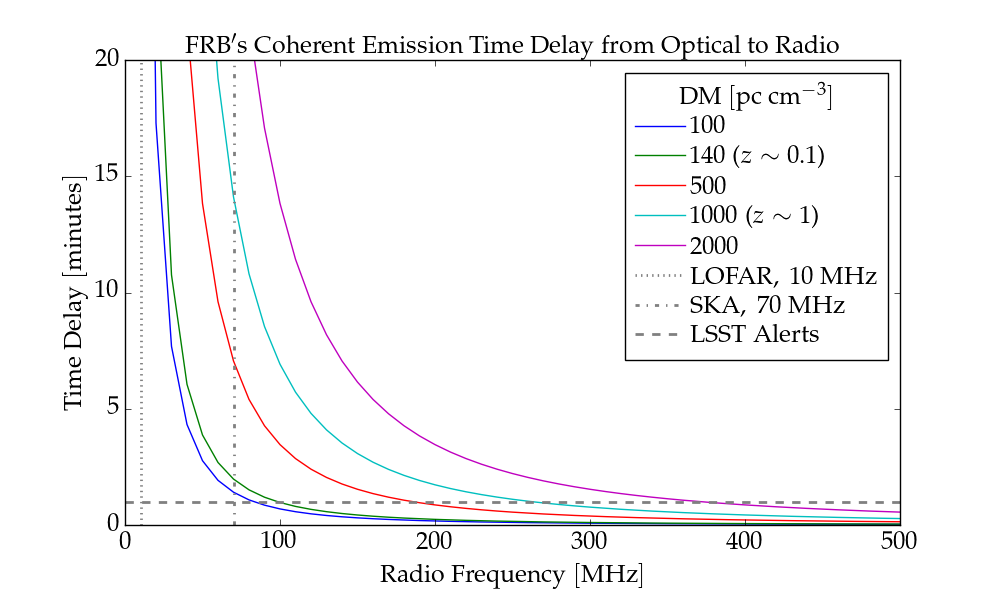
\includegraphics[width=12cm]{figures/frb_optical_delays.png}
\caption{The delay time (for coherent emission) between the arrival of the optical and radio photons due to cosmological dispersion, as a function of the frequency of the radio detector. The {\it lowest} frequency bands of the Square Kilometer Array (SKA\footnote{\url{www.skatelescope.org}}) and the Low-Frequency Array (LOFAR\footnote{\url{lofar.org}}) are marked with vertical dotted and dash-dotted lines, and the 1 minute timescale for LSST alert distribution with a horizontal dashed line. The delay time is $\Delta t = k_{\rm DM}\,DM\,(\nu_{\rm low}^{-2} - \nu_{\rm high}^{-2})$, where $k_{DM}=4.149$ $\rm GHz^2\ pc^{-1}\ cm^3\ ms$, ${\rm DM}$ is the dispersion measure in $\rm pc\ cm^{-3}$, $\nu$ is the low and high frequency bands of the observation, and $\Delta t$ is in $\rm ms$. We have used the range of FRB dispersion measures as observed by \cite{2018Natur.562..386S}. \label{fig:sci_frb}}
\end{center}
\end{figure}


\subsection{Summary of Science-Driven Broker Needs and Recommendations.}\label{ssec:sci_sum}

{\it Summarize the science-driven broker needs here, and perhaps also the 'Challenges Faced'. This section could also, e.g., use or modify Gautham's charted needs, or perhaps create as a new table matrix.}

Say something about how the < 5 min timescale will effect the project. 

Based on these science requirements, we make the following recommendations: 

\nrec
%{System}{Audience}{Phase}
{alerttimescale}
{Understand if there are any scientific uses cases requiring < 5min access to the alerts}
{What, if any, are the driving use cases for access to alerts in < 5 min}


% An overview of alert production in LSST, plans, policies and data products
% summary and pushing out to pther documents 
% Discussion about making PPDB public - not final so can't make public byu was a significant dosucssion    
% key findings, outcomes, 
\section{LSST Alert Production and Data Products (Eric)} \label{sec:alertproduction}

LSST's alert stream provides near-real-time updates about all the time-variable objects LSST detects.
LSST will find transient, variable, and moving objects using image differencing.
The alert production pipelines will take each new image and subtract a matched, coadded template image built from the last Data Release.
All sources---positive or negative---detected at 5$\sigma$ in the resulting difference image will be create \texttt{DIASources} and spawn alerts.  
Algorithmic details of the pipeline processing are described in LDM-151 \citep{LDM-151}.

The alert packets will include not only the triggering \texttt{DIASource} records but also a variety of contextual information to allow downstream science users to make rapid decisions about whether an alert is interesting.
This information includes the associated \texttt{DIAObject} record, any past measurements of the source in the last twelve months, and image cutouts.  
A full accounting of the alert packet contents is specified in the Data Products Definition Document \citep{LSE-163}.
Alerts are then streamed to community brokers and the LSST Alert Filtering Service (\S \ref{sec:archandtech}), and the \texttt{DIASource} and \texttt{DIAObject} records are stored in the Prompt Products Database (PPDB) for later query.

An expanded overview of the Alert Production system as well as discussion of the selection of community brokers is described in  LDM-612 \citep{LDM-612}.

During the broker workshop, several discussions emerged about the contents of the alert packet and whether they were optimal for enabling follow-up of transient events.
Topics included whether postage stamps should they be included in all alert packets, or if a public cutout service be sufficient; how the size of postage stamps affects classification; what variability characterization parameters should be included in alerts; whether classifiers have special needs for the types photometric redshifts computed in the Data Releases; and whether the association to three nearby static sky stars and extended objects was sufficient.

\nrec
{alertcontents}
{Review the contents of the Alert packets}
{DM Science should review the alert packet contents with the science collaborations, particularly the inclusion and size of the postage stamps, the variability characterization parameters, and details of the static sky association.}

Workshop participants discussed use cases for the realtime alert stream compared to the queryable PPDB, which contains the \texttt{DIASource} and \texttt{DIAObject} records in a relational database.
Currently, the PPDB is user-queryable by scientists with LSST data rights 24 hours after the data is taken.
This makes it likely that brokers would re-create databases like the PPDB from the alert packet contents.
A LONI from the DESC collaboration proposed replicating the PPDB on a daily basis.

\nrec
{ppdbpublic}
{Investigate making replicas of the PPDB available, and the PPDB contents public}
{DM Science should consider whether the PPDB can be considered a public data product and how technically it might be made available to brokers. 
}


\section{Experience from Precursor Surveys (Melissa) } \label{sec:precursor}

\MLG[inline]{"Experience from Precursor Surveys" section draft complete. Contact the following to verify text and invite as co-authors: Scott Barthelmy (scott@milkyway.gsfc.nasa.gov), Eric Christensen (eric@lpl.arizona.edu) and Matthew Graham (mjg@caltech.edu).}

%Ensure this section answers these questions: 
%- How are we planning to scale up from precursor surveys? e.g data rates, number of targets, scaling up of follow-up observations.
% - What are the challenges of scaling up to LSST rates?
% - Data Challenges?

This section summarizes the lessons that can be learned from three ongoing time-domain surveys and/or event-distribution networks: the Gamma-ray Coordinates Network, the Catalina Sky Survey, and the Zwicky Transient Facility.
The contents of this section are derived from invited presentations given by representatives\footnote{Thanks to Scott Barthelmy, Eric Christensen, and Matthew Graham for their talks at the workshop.} of each survey.

\subsection{Gamma-ray Coordinates Network ( {GCN})}
% MLG sourced GCN material from:
% LSST CBW Participants Drive > Presentations - Wednesday Afternoon > GCN_LSST_CBW_June2019_v8-2.pdf (public)
% LSSTBrokerWorkshop19 > SOC's Notes (private)

The  {GCN} evolved out of the  {BATSE}\footnote{Burst and Transient  {Source} Experiment; a part of  {NASA}'s Compton Gamma-Ray Observatory.} Coordinates Distribution Network ( {BACODINE}; 1993-1997), and is a complex system that's grown over time.
The  {GCN}'s self-described goal is to {\it ``Collect all  {transient} information from all sources and distribute it in real-time to all who want it"}, and it sits at the intersection of automated (real-time) and human-in-the-loop analysis.

Compared to the stream of  {LSST} alerts -- which will all have similar contents, be distributed within 60 seconds, and be world-public -- the  {GCN} supports a wide diversity of message types, contents, origins, filtering, and user-access options.
There are currently two categories of message types: notices (seconds to hours) and circulars (minutes to days)\footnote{A third category of reports, which had a timescale of days, has been discontinued.}.
Message contents can include positions, light-curves, images, spectra, temporal data, and/or telescope  {metadata} (pointing, thresholds).
Notices can be automatically generated by observatories, and circulars and reports can be submitted by a human (e.g., via socket connections, email).
Messages are automatically extracted, processed, and verified before circulation.
Filtering options for registered subscribers include brightness, significance, time since discovery, sky location, or source of the notice (e.g., gamma-ray burst, gravitational wave event, and $>$100 other types).
Access options include email, socket connections (including  {IVOA} VOEvent protocol), an online archival, etc.
The  {GCN} also supports the restriction of circulation to private networks (e.g., the  {LIGO}-VIRGO Collaboration's gravitational wave event notices in observing runs 1 and 2), and daily omnibus summaries.
The  {GCN} intends to receive and process at least a small subset of  {LSST} alerts that are relevant to its user base. 

{\bf Lessons learned from the  {GCN} include:}
considerable  {monitoring} infrastructure is required to ensure  {GCN}'s maximum system live-time ($>$99\%);
a parallel, stand-alone environment is necessary for testing new code and running stress-tests to assess system load and performance;
contents purity is ensured by implementing automatic file format checks every time files are edited;
and, of course, the importance of backing up the data, code, scripts, config files, and documentation.
% One takeaway seems to be that automation is never done!

\subsection{Catalina Sky Survey}
% MLG sourced Catalina material from:
% LSST CBW Participants Drive > Presentations - Wednesday Afternoon > Christensen_Eric_pdf2.pdf
% LSSTBrokerWorkshop19 > SOC's Notes (private)

This survey is optimized for the discovery and follow-up of Near-Earth Asteroids (NEOs), has been funded by  {NASA} since 1998, and is immensely successful: Catalina is credited for the discovery of almost half of all known NEOs.
This success can be attributed -- at least in part -- to this singular focus: all aspects of the survey are optimized for the scientific goal of  {NEO} discovery, and there are no competing interests.
This clear and resolute aspect garnered strong support from the wider  {NEO} follow-up community, which has compounded Catalina's success.
Out of necessity, the  {LSST} cadence must accommodate many science goals, but Catalina serves as a good example for brokers intending to focus on a singular  {LSST} science area or limited set of science goals. 

The Minor Planet  {Center} ( {MPC}) plays a key role by ingesting  {NEO} candidate reports and making them available to the community.
The  {MPC} has strict regulations on event reporting which lead to a $>$99\% purity rate of its database, but is in need of some modernization for the  {LSST} era, such as reducing processing latencies and improving database access.
These updates will enable the time-sensitive astrometric follow-up that is required to solve for asteroid orbital parameters.
For example, reducing the delay between initial  {NEO} detection and the creation of an ``actionable orbit" (from which follow-up observations can be planned) will be more scientifically productive, especially for faster-moving NEOs.

Towards this end, efforts are underway to develop the NEOfixer\footnote{See, e.g., \url{https://www.noao.edu/meetings/lsst-tds/presentations/Seaman_NEOfixer.pdf}}, an  {NEO} follow-up broker which will subscribe directly to  {NEO} candidates from the  {MPC}, not the  {LSST} alert stream ( {LSST} data is ingested to the  {MPC} daily).
The goal of NEOfixer is to strategically improve the quality of the  {NEO} catalog by optimizing worldwide\footnote{NEOfixers users include professional and amateur astronomers.}  {NEO} follow-up, scaled to the demands of future wide-area surveys like  {LSST}.
NEOfixer plans to offer subscribers an event prioritization that is customizable to a given observatory's location, aperture, and instrumentation (via a web interface and a direct socket), and the ability for users to report back their follow-up efforts in real time.

{\bf Lessons learned from the Catalina Sky Survey include:}
adopting a singular science focus can both facilitate the decision-making process for, and amplify the success rate of, a time-domain survey processing system;
interfacing with trusted community infrastructure enables community follow-up, which adds value to a data set;
providing customizable event prioritization for community follow-up helps ensure that resources are well matched to the needed observations.

% The NEO community is currently finding about 2000 new NEOs per year, and about 10-100 times more new main belt asteroids per year. Currently, about 2-3 candidate NEOs are discovered per real NEO.

\subsection{Zwicky Transient Facility ( {ZTF})}
% MLG sourced ZTF material from:
% LSST CBW Participants Drive > Presentations - Wednesday Afternoon > ZTF LSST Brokers.pdf
% LSSTBrokerWorkshop19 > SOC's Notes (private)

In operations since 2018, the  {ZTF} covers the northern sky ( {declination} $>$30 degrees) in filters {\it gri} to a 5$\sigma$ depth of $r$=20.5 mag with a variety of cadences, including up to six visits a night for some areas at some times \citep{2019PASP..131f8003B,2019PASP..131g8001G}.
Alert packets for difference-image sources are released in real time, have a similar format\footnote{Apache Avro; see \S~\ref{sec:archandtech}.} as the planned  {LSST} alerts, and are currently being consumed by at least $100$ unique sites via community brokers.
The primary follow-up system for the  {ZTF} project is the  {SED} Machine ( {SEDM}; \citealt{2018PASP..130c5003B}), a low-resolution Integral Field Unit spectrograph with a fully automated reduction  {pipeline}.
The  {ZTF} had publicly classified $1000$ supernovae as of mid-July 2019. 

{\bf Lessons learned from  {ZTF} include:}
API connections appear to be the most desirable mode for broker connections, which allow users to design their own interfaces;
as real-bogus scores evolve with new training, users will request that past events be re-classified;
the color information from {\it gri} only is insufficient for some science;
and finally that long alert IDs that are necessary due to the large number of detections but which are not human-friendly, e.g., ZTF19abctlvw will be generally derided\footnote{One suggestion was to use three 3-letter words in a row, e.g., ``catpawtoy", as that would provide $\sim$50 million memorable combinations.};
Since the  {ZTF} is still ongoing, surely there are more lessons to follow.



\section{Event Brokers for the LSST Alert Stream (Leanne \& Melissa)} \label{sec:lsstbrokers}

\MLG[inline]{``Event Brokers" section draft is complete. It is likely that the broker proposers might want to provide feedback on this summary.}

Compared to ZTF, the LSST will produce $\sim10$ times more alerts per image, obtain images at a slightly faster rate, generate alerts of a slightly larger size, and produce alerts for all standard single-visit images (whereas ZTF alerts are produced for the $\sim40\%$ of the images from the public surveys).
This adds up to a nightly data distribution that will be at least $\sim30$ times greater for LSST than for ZTF -- too big and too fast for the type of processing used in the past, e.g., bulk download and processing.
Specialized software systems -- event brokers -- will be required for the community to make scientific use of the LSST alerts, and turn them into scientific discoveries and a new understanding of the time-domain universe.

The LSST call for letters of intent for community alert brokers \citep{LDM-682} generated 15 letters of intent from teams proposing to receive the full LSST alert stream.
Three letters of {\it non}-intent were also submitted from teams who were developing associate software (such as TOMs) and/or were planning to do science related to the alerts but were not actively developing a broker.
Representatives of all 18 letter-writing teams were invited to participate in the CBW and contribute a presentation.
The Data Management System will be capable of transmitting at least five full streams out of the alert distribution system \citep{LSE-61}.
It is the role of the LSST Science Advisory Committee (SAC) to evaluate the proposals and decide which brokers will receive the full stream.
The SAC assessed the letters of intent and, in December 2019, invited all 15 teams to submit full proposals (due June 2020).
The full criteria for broker evaluation are provided in \citet{LDM-612}; briefly, these criteria include the proposals' scientific potential in terms of range and impact; their ability to reach and serve a diverse community; and/or their integration and/or complementary with other software systems and platforms. 

The proposing teams represented eight countries, with eight proposals from the USA, five from the UK and Europe, one from Chile, and one from South Africa; there were thirteen/two proposals from the northern/southern hemisphere, respectively.
Eleven proposals stated that they would need the full stream, and four stated that they would want or could use stream that was pre-filtered based either on sky region (i.e., to match their follow-up capabilities or science goals) or object type (e.g., moving or stellar objects).
Six proposals identified as science-specific; all six were interested in alerts for a certain object type (e.g., moving objects, transients, variable stars), and three were also only interested in alerts in certain locations (e.g., transient host type or sky area).
Of the nine proposals that identified as general, five identified as having a focus on non-moving objects (i.e., transients and variables), and four identified as having a focus on method (e.g., machine learning techniques).
With respect to cooperative interaction between brokers, two proposals stated they were already working together, with one passing ZTF alerts to the other.
A further three proposals mentioned specific plans to interact with other brokers, and during the meeting a vision for a ``broker ecosystem" with peer-to-peer networking to enable science was a common discussion topic (see Section \ref{sec:conops} for more on this).
In terms of development status, six proposals identified as being at the conceptual stage, three identified as being in active code development, and six reported that they were already processing ZTF alerts and supporting science (either in real time from the ZTF alert stream, or from bulk downloads). 
Seven of the broker proposals -- and one letter of non-intent -- have publicly available documentation about and/or user interfaces to their alert processing systems; links and citations are provided in Table \ref{tab:brokers}.
The letters of non-intent focus on providing external platforms for scientific analysis, such as those discussed in Sections \ref{ssec:interfaces_other} and \ref{ssec:interfaces_brokers}.

\begin{table}[h!]
\label{tab:brokers}
\centering
 \begin{tabular}{ll} 
 \hline
 Event Broker & Access, Documentation, or References \\
 \hline\hline
 ALeRCE & \url{alerce.science} \\
 AMPEL & \protect{\citet{ampel}} \\
 ANTARES & \url{antares.noao.edu},\ \protect{\citet{2016SPIE.9910E..0FS}}\\
 Fink & \url{fink-broker.readthedocs.io} \\
 Lasair & \url{lasair.roe.ac.uk},\ \protect{\citet{2019RNAAS...3...26S}} \\
 MARS & \url{mars.lco.global} \\
 SASSy & \url{sassy.as.arizona.edu/sassy/ztf} \\
 Pitt-Broker & \url{pitt-broker.readthedocs.io} \\
 \hline
 \end{tabular}
\end{table}

In terms of functionality, all fifteen proposing teams stated their broker would be cross-matching the LSST alerts to external catalogs (mostly static-sky catalogs, but some to archival time-domain catalogs), and some mentioned cross-matching to time-domain events from other real-time sky surveys.
This common need prompted a discussion about how brokers could work together to build and share a centralized cross-matching service to reduce redundancy in effort and computational resources.
Almost all teams stated that their broker would be using light curves for photometric classification, with a variety of methods such as feature extraction, template fitting, and machine learning.
Most intended to have these light curve analyses operating in real time to filter the stream, and a few teams were focused on very rapid probabilistic classification of objects for follow-up observations. 
Some brokers are planning to have the light curve analysis tools available to users to apply to aggregated alerts data in an ``non-streaming" mode (i.e., not embedded in a filter). 
A few brokers intend to focus their light curve analysis tools on specific types of objects, such as variable stars or moving objects.
At least four broker teams mentioned accessing the LSST Science Platform (Section \ref{sssec:interfaces_lsp_brokers}) to obtain additional information about events from the Prompt Products Database or the Data Release catalogs, which would assist with their classifications.

With respect to user access, most brokers plan to provide a web-based (in-browser) query interface, and many mentioned providing APIs, JupyterHub or notebook access, data export services (e.g., table downloads, nightly tarballs of classified alerts).
Only a few brokers are planning to provide provenance functionality so that users can model the selection effects of the broker's algorithms.
Provenance is necessary for, e.g., analyses of events rates or cosmological studies, but is quite a challenge to provide.
About half of all broker proposals include functionality for users to define filters and receive alerts in real-time (and all brokers will have their in-house filters as well).
At least one cloud-based broker is looking towards a ``freemium" cost model and making constainerized instances of their filters available to anyone. 
About half of all broker teams stated an intention to release the results of their filters and classification as a stream of annotated alerts, and a couple intend to post public lists of objects prioritized by their need for follow-up.
This output would be sent to, e.g., TOMs or other object-aggregating services\footnote{E.g., the Transient Name Server \url{wis-tns.weizmann.ac.il}}.
With respect to follow-up, only a couple of brokers intend to have self-contained TOM-like functionality, interface directly with follow-up facilities, and allow users to trigger observations (TOMs are described in Section \ref{sec:followup_toms}).
Comparing this list of planned broker functionality to the summary list of science-driven needed functionality at the end of Section \ref{sec:science}, we can see that there are no potential needs that remain uncovered by the full suite of broker proposals.

{\bf Challenges faced by broker developers include:} scaling their alert processing from the ZTF stream to LSST; writing code for LSST-formatted alerts which will be different from ZTF alerts; how to provide provenance for users who need it; identifying their role within an evolving ``broker ecosystem"; reducing redundancy in algorithmic development (e.g., how to develop and share a cross-match service); and understanding what types of pre-filtered streams might be an option (from LSST and from other brokers).
Naturally, some of these challenges overlap with those identified from the science drivers discussed in Section \ref{sec:science}.

\noindent {\bf To address these challenges, we make the following recommendations:}

\nrec{System}{Audience}{Phase \textcolor{red}{Leanne was going to remember what was meant by this.}}

\nrec{System}{Organize another meeting for the events brokering community}{Another face-to-face meeting for all those involved in brokering LSST alerts should be planned (to coincide with test alerts from commissioning?). This meeting should include not just the five selected for full stream transmission, but also representatives of downstream brokers, applied algorithms, science platforms, follow-up systems, etc.}

%5% How does this interact with technical decisions about stream contents, latencies, broker hosting location, etc.? 
%%% What test data products are needed by brokers? ZTF is the precursor test facility for brokers to scale up on. The NSF is funding ZTF for this reason. What is the timeline for closer integration during commissioning?
There are furthermore three recommendations introduced in Section \ref{sec:conops} which are relevant to addressing the above challenges: \textcolor{red}{REC-X} to further define the test streams during commissioning; \textcolor{red}{REC-X} to investigate the types of filtered streams that LSST could provide; and \textcolor{red}{REC-X} to investigate options for expanding access to the alert stream (to potentially allow transmission of $>5$ full streams).


% % % % % % % % % % % % % % % % % % % % % % % % 
%%% MLG: Below are suggestions for content in this section that I didn't much cover, and why.

%%% Provide a summary of the emergent network of brokers, peer-to-peer alert transport, ``downstream" brokers, "hierarchical event brokers", and the ecosystem with other platforms and TOMs.
%%% MLG: just cited Section 11, "Alert Ecosystem in LSST Operations", which is the more relevant place for such information.

%%% What is the minimum added values that brokers need to add to be considered?
%%% MLG: I wasn't sure what this was in reference to... if it's about the criteria for broker selection, that's covered in paragraph 2.
% Algorithms for processing of the alert stream
% summary of the talks, challenges 
% collaborative XMatch - unconference 
% how they work with broker proposals 
\section{Algorithms for alert stream processing (Leanne)} \label{sec:algorithms}
Algorithms for real-time transient filtering and event classification range from simple filters that apply 1-dimensional cuts on attributes in the Alert packet through to complex machine-learning based classifiers. 

% filtering (simple filters and  machine-learning based), and characterization. 


Integration and cross-match with other survey data.

Challenges involved in mining the LSST alert stream

Reference other papers 



\section{User Interfaces (Melissa, Gregory)} \label{sec:interfaces}
% Resources used:
% https://community.lsst.org/t/lsst-answers-to-community-broker-faqs/3780
% LSST CBW Participants Drive > Presentations - Wednesday Morning > Bellm_AP_overview_190619.pdf
% The SOC's google doc full of notes from the CBW

% Make sure the contents address the following:
% How will the scientific community interact with community brokers and access the LSST data products? 
% How will community brokers interface to science platforms, data archives 
% How can pipelines for User-Generated data processing and analysis interface with the LSST alert stream
% Identified needs and connect them to science, i.e., to enable X science - need Y science.

\MLG[inline] {"User Interfaces" section draft contains all of my contributions and is ready for input from others.}

This section discusses user interfaces that enable science by providing access to the LSST data products, user- or broker-generated data products, and external (archival) data.
This includes brokers as users of the alert stream, individuals as users of the brokers, and both brokers and individuals using the Rubin science platform or other data archives.
The contents of this section were generated from invited presentations and discussion sessions at the workshop\footnote{Thanks to Knut Olsen, César Briceño, Stéfan van der Walt, Austin Riba, and the broker proposal teams for their talks relating to science platforms and interface development.}.

\subsection{IVOA}\label{ssec:interfaces_ivoa}

\MLG[inline] {"IVOA" subsection of "User Interfaces" needs contributions from someone who knows the content.}

More information about VOEvents, the  {IVOA} (International Virtual Observatory Alliance), and  {VTP} (VOEvent Transport Protocol) can be found in \citet{2011ivoa.spec.0711S} and \citet{2017arXiv170901264A}.


\subsection{The Rubin  {Science Platform}}\label{ssec:interfaces_rsp}
% {\it What will the interface between the RSP and Community Brokers look like for users? How about for the LSST Alert Filtering Service?}

The Rubin  {Science Platform} ( {RSP}) is a collaborative research environment that provides access to   LSST data products and services for all science users and project staff.
The  {RSP} provides a set of integrated web applications and computational resources deployed at   LSST Data Access Centers (DACs).
The  {RSP} is composed of three main aspects, each of which could be considered a "user interface":
(1) Portal, for exploratory search, analysis, and visualization of the   LSST archive;
(2) Notebook, for in-depth next-to-the-data analysis with pre-installed and custom libraries that enable the creation of added-value user-generated data products, without the need for users to download large volumes of data; and
(3) Web  {API}, enabling remote access to the   LSST datasets and services using community-accepted formats and protocols\footnote{A ``VO First" strategy has been adopted, which means that IVOA protocols will be used wherever possible}.
More information about the  {RSP} design can be found in \citealt{LSE-319, LDM-542}.

Below is described alerts-related interfaces with the  {RSP}, from the perspective of individual users (\S~\ref{sssec:interfaces_rsp_individual}) and community brokers (\S~\ref{sssec:interfaces_rsp_brokers}).

\subsubsection{Individual Users' Interfaces to the  {RSP}}\label{sssec:interfaces_rsp_individual}

Most scientists will access   LSST alerts via community brokers.
Although it will be possible for users to ingest a set of broker-filtered alerts to their user account in the   LSST  {Science Platform} ( {RSP}) -- and note that this would be subject to the same data storage limits as any other uploaded data set -- a more efficient use of the  {RSP} would be to directly access the original prompt data products from which the alert packets are derived (i.e., the images and catalogs described in Section 3 of \citealt{LSE-163}).
The contents of the alerts and the  {PPDB} are essentially identical, with the main difference being timescale: alerts are released within $60$ seconds of image readout, whereas the prompt products are available within $24$ hours.

Some scientists might instead use the   LSST  {Alert} Filtering Service, which will provide basic, limited capacity access to the   LSST alert stream, and is sized to allow 100 simultaneous user-generated filters to return 20 alerts per visit (Section 2.2.4, \citealt{LSE-61}).
The   LSST  {Alert} Filtering Service is still in development, but is expected to provide VOEvent format alerts (or similar; Section 3.5.2 of \citealt{LSE-163}).

It is expected that users of the   LSST  {Science Platform} ( {RSP}) will be able to define an alert stream filter in the  {RSP} environment and have it installed in the   LSST  {Alert} Filtering Service, which is separate from the  {RSP}\footnote{RSP facilities are for analysis and queries of the   LSST data products and not for continuously-running processes such as alert stream filters.}.

Users may receive their filtered alerts from the   LSST  {Alert} Filtering Service by, e.g., a simple User Interface provided in the  {RSP} via the Portal Aspect (Section 3.9 of \citealt{LDM-542}; Section 2.9.5 of \citealt{LDM-554}), and/or a direct connection using standard  {IVOA} protocols to a third-party system (e.g.,  {VTP} to a private server).
It is important to note that although it should be possible to query the Alerts Database from the  {RSP} \citep{LDM-542}, the Alerts Database might only support queries by alert  {ID}. 

\subsubsection{Community Brokers' Interfaces to the  {RSP}}\label{sssec:interfaces_rsp_brokers}

External entities (e.g., brokers) may interface with the  {PPDB} via the Web  {API} aspect of the   LSST  {Science Platform}, and use the  {TAP} interface\footnote{More information about  {TAP} can be found at: \url{http://www.ivoa.net/documents/TAP/} and \url{https://www.cadc-ccda.hia-iha.nrc-cnrc.gc.ca/en/doc/tap/}.} to query the  {PPDB} catalogs by, e.g., using {\tt DIAObject} or {\tt DIASource} IDs from the alert packet as keys (\citealt{LSE-319, {LDM}-542, {LDM}-554}).
The  {PPDB} catalogs are updated with new data within {\tt L1PublicT} of image acquisition (currently 24h; \citealt{LSE-29}). 


\subsection{External Science Platforms and Archives}\label{ssec:interfaces_other}
% Materials used
% LSST CBW Participants Drive > Presentations - Thursday Afternoon > Stefan van der Walt - SkyPortal
% LSST CBW Participants Drive > Presentations - Thursday Afternoon > DataLab_CBW.pptx
%{\it Integration with other science archives or platforms, e.g Datalab, Canadian LSST Advanced Science Platform, others. Interfaces to data archives such as the CADC, etc.}

As astronomical data sets grow in size and complexity, it becomes increasingly necessary to co-locate the data with the tools and compute resources for scientific analysis.
The user interfaces for these systems, the science platforms, will play critical roles in the analysis of new and archival data sets, enabling science and expanding discovery space for a broad cross-section of the community \citep[e.g.,][]{2019arXiv190305130O}.
The  Rubin Science Platform is just one example of an astronomical science platform serving as a user interface to a data archive or an alert stream, and some community brokers and TOMs could be considered science platforms.
It is expected that non-Rubin science platforms may want to offer users the opportunity to access the LSST alerts or other LSST data products via, e.g., Web  {API}, without that platform having to ingest the LSST data into its database.

In general, it is common for science platform's user interfaces to be a browser-based web front-end built on a web  {API}, and desirable that interfaces be modular and customizable to the user -- or a user groups' -- science needs.
The  {TOM} Toolkit (discussed in \S~\ref{sec:followup}) is one example of a customizable user interface.
SkyPortal\footnote{\url{https://skyportal.io}} \citep{skyportal2019}, designed as a platform for time-domain survey data from  {ZTF} and eventually  {LSST}, allows users to customize how the data for a given object is rendered.
For example, interactive plots of light-curves and  {postage stamp} images from an alert packet can appear alongside user-supplied spectra and/or comments.

The  {NOAO} Data Lab \citep{2019arXiv190800664O} has built its user interfaces on the guiding principle of enabling efficient exploration through which users can develop intuition through interaction with catalogs, images, and spectra, and have this lead to discovery.
Embedded data visualization tools play a big role in this, and they are offered to users via, e.g., pre-installed libraries that can be called from Jupyter Notebooks.
The Data Lab currently hosts public datasets from massive ground-based surveys in the  {NOAO}  {Archive}, and also provides a platform for  {ANTARES} filter development and testing, and for the analysis of  {ZTF} alerts that pass filters installed in  {ANTARES} (also via browser-based notebooks). 

The Canadian Astronomy Data  {Center}\footnote{\url{http://www.cadc-ccda.hia-iha.nrc-cnrc.gc.ca/en/}} ( {CADC}) offers specialized astronomy and data management expertise to the worldwide community, to support data access to and analysis of very large astronomical data sets (many, but not all, of which are from Canadian facilities).
The  {CADC}'s web browser interface allows users to search its archival collection by spatial, temporal, spectral, observational constrains (e.g., proposal keywords, instrumental filter), or  {calibration} level (e.g., raw, calibrated, or products like stacks).
Authorized users can also create virtual machines (VMs) and submit batch processing jobs and share the results.
The  {CADC} is exploring ways to partner with a broker, ingest alerts (potentially subsets of alerts, and/or with greater latency), serve them to the community, and enable user activities that add value to the alerts via co-analysis with the  {CADC}'s other archival resources.


Common themes regarding science platform (and broker/TOM) development which enhance the user experience emerged during the presentations and discussion sessions at the workshop, and they include:
\begin{itemize}
\item {\it Open Development} -- to encourage collaboration in the community and ensure that the tools developed are widely applicable
\item {\it Open  {Source}} -- to reduce redundancy in tool development and enable customization
\item {\it Open Access} -- to ensure tools and data are accessible to as broad a community as possible (i.e., user accounts that are authenticated, but freely available)
\item {\it Customizability} -- to enable broad adoption of tools, they should be adaptable to different science use-cases
\item {\it Provenance} -- packages and tools can be restored to earlier versions for testing; tracking user contributions to tools and derived data products for attributing credit properly
\item {\it Documentation} -- tools need to be well tested and documented for broad adoption
\end{itemize}

\subsection{Brokers, TOMs, and Follow-up Resources}\label{ssec:interfaces_brokers}

Each community broker defines its own user interfaces through which individuals can access a broker's products, such as alert stream filters, value-added data products, or queryable database.
This access is typically via web browsers or desktop clients.
Currently, at least three brokers ( {ANTARES}, ALeRECE, and Lasair) have publicly accessible websites through which users may view lists of results from filtered streams, query the database, and visualize alert packet contents (e.g., light curves, image stamps, and any user-uploaded data such as spectra, classifications, or redshifts).
Additionally,  {ANTARES} has a client\footnote{\url{https://gitlab.com/noao/antares/client}} for command-line based interaction with the live alert stream, Lasair offers a set of {\sc Jupyter} notebooks\footnote{\url{https://lasair.roe.ac.uk/jupyter}} for users to work with alerts, and ALeRCE has released an  {API}\footnote{\url{https://github.com/alercebroker/usecases/tree/master/api}} for access to their databases of alerts and postage stamps.

Similarly to brokers, TOMs such as the Las Cumbres Observatory  {TOM} Toolkit \citep{2018SPIE10707E..11S} are also deployed for browser-based access by users.
The TOMToolkit codebase is in {\sc Python} and {\sc Django}, the latter of which has many pre-existing modules that enable a developer to easily customize their interfaces and add functionality appropriate for the  {TOM}'s science goals.
The customized  {TOM} can then be deployed via, e.g., {\sc Heroku}. More details about TOMs are provided in \S~\ref{sec:followup_toms}.

Interfaces from brokers and TOMs to follow-up resources is one of the common science-driven needs discussed in \S~\ref{sec:science}.
The Zwicky Transient Facility and the The Las Cumbres Observatory have been sending observation requests to their follow-up telescopes from their respective browser-based  {TOM} systems for at least a few years (e.g., \citealt{2018SPIE10707E..11S}).
The user interfaces for this functionality are drop-down selection boxes embedded in the website from which a user can set the observational parameters (e.g., target, instrumental  {configuration}, time window, integration, repeat cadence), and a button to add the request to the telescope's queue.
The interface typically also includes, e.g.,  {airmass} curves for the target of interest at the follow-up facilities, to assist the user in setting the observation request.
An example of the software system which manages these observation requests is the Astronomical Event Observing Network\footnote{\url{https://lco.global/aeon}},  {AEON}, which is discussed further in \S~\ref{ssec:followup_networks}.

\textcolor{red}{Get a reference, a website at least, for the following two statements or just remove them.}
As a final example, the Gemini Observatory's  {API}, the Observing Tool, has long been used by staff and observers to submit observing blocks to the Gemini queue, including targets of opportunity.
A new version of the tool is under development to enable web-based user access and integration with  {AEON} and  {TOM} systems.


\subsection{Challenges in User Interface Development}\label{ssec:interfaces_challenges}

During the discussion sessions at the workshop, the following challenges in user interface development were identified:
\begin{itemize}
\item the authentication and authorization of user accounts
\item preserving   LSST data rights in a data-sharing environment 
\item coordination of authenticated user accounts between platforms
\item obtaining the computational resources required to support user activities and large data sets (e.g., query interfaces)
\item community-wide adoption of standards to enable cross-platform interaction (e.g., querying external archives from a  {TOM})
\item data visualization tools for very large data sets
\end{itemize}

% {\it To address these challenges, we make the following recommendations:}


\section{Architecture and Technologies (Eric) } \label{sec:archandtech}

\subsection{Streaming technologies for high-rate alert steams}

LSST has baselined the open-source distributed streaming platform Kafka\footnote{\url{https://kafka.apache.org/}} for distributing its ten million nightly alerts.
Kakfa is a low-latency, fault tolerant message queue used widely in commercial industry.
In addition to on-premises hosting, managed installations of Kafka are available on commercial cloud providers such as AWS\footnote{\url{https://aws.amazon.com/msk/}} and the Confluent Cloud\footnote{\url{https://www.confluent.io/confluent-cloud/}}.
Scale tests during LSST construction have shown that Kafka meets LSST's performance requirements \citep{DMTN-028}. 

The baselined alert serialization is Apache Avro\footnote{\url{https://avro.apache.org/}}, a open-source schema-ed binary format widely used with Kafka.

Since 2018 the ZTF project has been distributing LSST-like alerts to community brokers using Kafka \citep{Patterson:19:ZTFAlerts}.
ZTF averages 1025 alerts per image, and takes one image every 40 seconds.
Each ZTF alerts is about 70 kB (although ZTF alerts contain less catalog information than LSST alerts, they have an extra cutout and an uncompressed Avro schema). 
This means that the LSST alert stream is a factor of 11.5 larger in number of alerts per second and a factor of 13.4 larger in data rate than the total ZTF alert stream.
Only 40\% of the ZTF alerts contribute to the public alert stream.

Some brokers demonstrated or discussed tools for stream processing of ZTF and LSST alerts.
The Fink broker is built on the open-source Spark Streaming library.
ANTARES built a custom Python-based filtering system.
AMPEL using a multi-stage custom processing system that annotates, cross-matches, and filters alerts.

\subsection{Databases}

Many brokers currently running on ZTF alerts are storing alerts (or data extracted from alerts) in databases.
Popular choices include both relational databases such as Postgres as well as NoSQL solutions such as MongoDB.
Several brokers also retained the original ZTF alert packets in an object store or similar.

As brokers prepare for LSST scale they are considering additional open-source database technologies such as Apache Cassandra and Apache Ignite.
Managed cloud databases such as Google BigQuery offer a cloud-native approach. 
LSST's Qserv \citep{2011Wang:2011:QDS:2063348.2063364} is another potential candidate.

\subsection{Hierarchical or networked systems of brokers}

For both scientific and technical reasons we expect brokers, TOMs, and related systems to develop into a networked ecosystem, where alerts may pass from LSST through multiple brokers before reaching a science user or followup facility.
Broker systems along the way may add value through classification or crossmatch and enable more effective filtering to subsets of events of interest.
The forwarding function itself was envisioned by the original VOEvent broker concept, and helps relieve the bandwidth pressure on the transfer from the LSST Data Facility.

We discussed how LSST might facilitate the development of such broker networks.
One possibility would be to favor selection of brokers who are willing to forward alerts to other ``downstream'' brokers.

An alternative would be to investigate ways for LSST to supply alerts directly to a larger number of community brokers.
This might be accomplished by allocating more outbound bandwidth from the LSST Data Facility, providing pre-filtered streams or ``light'' alerts with reduced contents, setting up simple alert forwarding systems in other locations, increasing alert transmission latency, and/or providing copies of the alert stream or PPDB in the cloud.

Having some brokers co-located at  the LSST Data Facility would also ease outbound bandwidth constraints.

\LPG[inline]{I'm not sure it would ease the outbound bandwidth as there would be several downstream brokers who would pull a filtered stream and  a large number of users connecting to the broker at the LDF and pulling filtered streams. It is not clear whether it would reduce or increase the outbound bandwidth, It would change the access patterns. }

At present agreements to co-locate would be developed by the broker teams and the LDF directly, without LSST Project involvement.


\nrec{expandstreams}
{Investigate possibilities for expanding alert stream access}
{Investigate options for providing alerts to a larger number of brokers. 
Determine trade space of cost, science loss due to reduction in alert stream contents, and science gain due to expanded access to alerts.}

\subsection{Cloud Deployment}

As outlined in the  recent Astro2020 APC White Paper ``Astronomy should be in the clouds'' \cite{Smith:2019gqn}, commodity cloud computing, as provided by commercial vendors such as Amazon, Google, and Microsoft, has the potential to fundamentally change the way data from astronomical large astronomical surveys such as LSST, WFIRST, etc, is processed and served to a global community. 

Commercial clouds provide the potential for on-demand, easily scalable analysis workflows for datasets of LSST scale and beyond.  
Science users could directly provision the resources required for their analysis task and take advantage of the high bandwidth within cloud regions to access the entire LSST alert stream.  
Additionally, cutting-edge industrial tools provide increasingly accessible means of processing petascale datasets;
commercial cloud databases like BigQuery could provide performant hosting of a PPDB clone, for instance.
However, issues of cost, training, and accessibility remain to be explored.

\nrec{ppdbincloud}
{Investigate the possibility of hosting the alert stream and/or PPDB in the cloud}
{Investigate the possibility of providing a cloud-hosted version of the alert stream and/or PPDB that is publicly accessible, including understanding what latency would be acceptable and how  this interacts with other LSST requirements.}
\section{Followup Tools and Services (Melissa)} \label{sec:followup}
% Materials used
%LSST CBW Participants Drive > Presentations - Friday Morning
%SOAR_AEON_Presentation_June2019.pdf
%LCO LSST Broker LONI Presentation

\MLG[inline]{Section status: MLG preliminary text generation in progress. Should invite Cesar and Rachel and Austin to contribute here.}

\smallskip

\noindent
{\it Ensure this section contains:
\begin{itemize}
    \item How will automated follow-up be enabled?
    \item How will brokers and science platforms integrate and coordinate with
follow-up observing facilities and networks?
\end{itemize}
}

Time-domain science with LSST will benefit significantly from additional observations enabled by \emph{follow-up} facilities and services, and some science goals absolutely require follow-up data. Enabling rapid follow-up observations is one of the main science-driven needs for community brokers, as described in Section \ref{sec:science}. In these sessions we explored how to enable automated, real-time integration of the LSST alert stream with follow-up networks and target observation managers (TOMs).

\subsection{Follow-up Networks}

Astronomical Event Observing Network\footnote{\url{https://lco.global/aeon/}} (AEON) is the software architecture that allows for the automatic queue scheduling of requested follow-up observations, and is currently in development between the Las Cumbres Observatory and SOAR Telescope. With AEON, accepted proposals may submit their observation requests via API, thereby allowing the auto-generation of follow-up observations by, e.g., TOMs, for targets which meet certain pre-defined criteria. For example, three consecutive epochs of multi-band photometry show a faint but rapidly rising blue transient associated with a low-$z$ host galaxy. A request for a low-resolution spectrum could be automatically generated with, e.g., a 2-day window and intermediate priority, and submitted to the SOAR scheduler. In this process, AEON is the software that enables the TOM to communicate directly with the SOAR queue. 

\MLG[inline]{from here we could get more detailed on how AEON works -- Cesar's talk has many details -- but I'll leave that for later.}

Some of the main challenges faced by such follow-up networks are minimizing overheads (e.g., idle time, network delays, observations that run over their scheduled time window), ensuring the necessary instrument and telescope constraints can be specified in the TOM, support for moving objects, and the automatic reduction and resubmission of processed follow-up data from the telescopes back to the TOMs. 

\subsection{TOMs}

\smallskip
\noindent
{\it Ensure this section contains:
\begin{itemize}
    \item Will TOMs be run as a service that brokers can connect to?
    \item Will brokers integrate TOMS into their platform astropy style?
\end{itemize}
}

In the LSST era, sample sizes for transients and variable stars will increase by at least an order of magnitude for even the rarest sub-groups, and likely much more, as will the diversity in classification types -- all of which will have different science-driven needs for follow-up observations and analysis. Target Observation Managers (TOMs) are currently being developed to meet this challenge. TOMs could be considered as a specialized sort of science platform that is driven by time-domain science and follow-up observations: software to coordinate observing programs and keep track of target samples, observations, and derived data products. 

The Las Cumbres Observatory's TOM Toolkit aims to provide an open-source modular software package that enables astronomers to build TOM systems and customize them for a given science goals. These software packages provide core functions for common tasks and well-defined interfaces to allow the TOM to communicate with, e.g., brokers and follow-up networks. By making this open-source, the hope is that a community of TOM users will arise and support each other in the further development and use of TOM systems. 

In the example above of a faint but rapidly rising blue transient, the TOMs role might be ingesting the associated alerts from the broker, performing additional tasks to add information to the target (e.g., cross-matches with external catalogs, light-curve feature fits, adding tags or labels, assigning to science-based samples), evaluating a target's need for science-driven follow-up, auto-generating follow-up observation requests and submitting them to follow-up networks, and ingesting the follow-up data (e.g., spectra) and performing analysis (e.g., spectral typing) which then further informs the need for science-driven follow-up.

\MLG[inline]{Some of the main challenges faced by TOMs are ... (MLG is unsure, the LCO TOM Toolkit talk didn't have a list like the AEON talk did... but surely they could contribute here).}

To  address these challenges, we make the following recommendations: 
% Putting it all together in here - how do we run it all in operations
\section{Alert ecosystem in LSST Operations (Leanne)} \label{sec:conops}
One of the key motivators for this workshop was to develop a vision of an integrated global ecosystem for transient science in the LSST era. Here we describe the concept of operations not just for LSST alert stream but but the whole system integrated ecosystem for transient science in the LSST Era. 


\subsection{LSST Commissioning}
Reference relevant commissioning documents

\subsection{LSST Operations}
Reference relevant commissioning documents


%%% Recommendations
To address these challenges, we make the following recommendations:

\nrec{teststreams}
{Investigate the possibility of providing test streams for broker testing}
{Investigate the possibility of the project providing test streams of alerts for brokers and downstream TOMS to enable broker development, data challenges, and operations rehearsals
}

\nrec{usercomputing}
{Provide a more robust definition of “10\% of the LSST computational system”}
{Provide a more robust estimate of what “10\% of the LSST computational system” means, so that the scientists and future users can begin to figure out whether that will meet their needs, and prepare grants/proposals.
}

\nrec{filteredstreams}
{Investigate the possibility of providing filtered streams}
{Clarify if/how the project could provide filtered streams, e.g
Simple filters: RA/DEC, Magnitude, Spuriousness cuts?
Image-free streams of alert packets?
sources associated with past alerts?
and provide estimate of how much the stream volume is reduced by these options.
}

\nrec{expandedaccessstream}
{Investigate options for expanding access to the alert stream}
{There is clear demand for expanding (near-) real time access to the full alert stream to ~tens of users, and a number of ways to get there:
less information in alerts
accepting longer latencies (5 minutes, not 60 seconds?)
network of mirrors forwarding the stream
cloud hosting}
% Summary of the key take-aways and findings 
% Actions, future work, next steps
\section{Followup and Conclusions (Leanne)} \label{sec:conclusions}

 This workshop provided a unique opportunity to bring together representatives of the LSST project, Science Collaborations proposers of community brokers and follow-up facilities, and industry to build a vision for an integrated global ecosystem for transient science with the LSST alert stream.
 
 \LPG[inline]{Summarize some of the new concepts and ideas that emerged and the implications for the project}
 
 \LPG[inline]{ Summarize the next steps that the LSST project will take in response to the outcomes of this workshop.}

\acknowledgments
This material is based on work supported in part by the National Science Foundation through Cooperative Agreement 1258333 managed by the Association of Universities for Research in Astronomy (AURA), and the Department of Energy under Contract No. DE-AC02-76SF00515 with the SLAC National Accelerator Laboratory. Additional LSST funding comes from private donations, grants to universities, and in-kind support from LSSTC Institutional Members.

This research has made use of NASA's Astrophysics Data System Bibliographic Services.
% \facility{LSST}

%\appendix
% Remove this when you strart your paper
%\input{appendix}

	% Include all the relevant bib files.
% https://lsst-texmf.lsst.io/lsstdoc.html#bibliographies
%\section{References} \label{sec:bib}
%\bibliographystyle{plainnat}
\bibliographystyle{yahapj}
\bibliography{brokers}
%\bibliography{brokers}

% Make sure lsst-texmf/bin/generateAcronyms.py is in your path
\section{Acronyms} \label{sec:acronyms}
\addtocounter{table}{-1}
\begin{longtable}{p{0.145\textwidth}p{0.8\textwidth}}\hline
\textbf{Acronym} & \textbf{Description}  \\\hline

 &  \\\hline
AEON & Astronomical Event Observatory Network \\\hline
AGN & Active Galactic Nuclei \\\hline
AMPEL & Alert Management, Photometry and Evaluation of Light curves \\\hline
ANTARES & Arizona-NOAO Temporal Analysis and Response to Events System \\\hline
API & Application Programming Interface \\\hline
AURA & Association of Universities for Research in Astronomy \\\hline
AWS & Amazon Web Services \\\hline
B & Byte (8 bit) \\\hline
CA & Control (or Cost) Account \\\hline
CADC & Canadian Astronomy Data Centre \\\hline
DE & dark energy \\\hline
DEC & Declination \\\hline
DESC & Dark Energy Science Collaboration \\\hline
DM & Data Management \\\hline
DMTN & DM Technical Note \\\hline
EPO & Education and Public Outreach \\\hline
GCN & GRB Coordinates Network \\\hline
HTC & High Throughput Computing \\\hline
IVOA & International Virtual-Observatory Alliance \\\hline
LDF & LSST Data Facility \\\hline
LDM & LSST Data Management (Document Handle) \\\hline
LIGO & Laser Interferometer Gravitational-Wave Observatory \\\hline
LSE & LSST Systems Engineering (Document Handle) \\\hline
LSST & Legacy Survey of Space and Time (formerly Large Synoptic Survey Telescope) \\\hline
LSSTC & LSST Corporation \\\hline
MPC & Minor Planet Center \\\hline
NASA & National Aeronautics and Space Administration \\\hline
NEO & Near-Earth Object \\\hline
NOAO & National Optical Astronomy Observatories (USA) \\\hline
PPDB & Prompt Products DataBase \\\hline
RA & Right Ascension \\\hline
RSP & Rubin Science Platform \\\hline
SAC & Science Advisory Committee \\\hline
SC & Science Collaboration \\\hline
SED & Spectral Energy Distribution \\\hline
SLAC & SLAC National Accelerator Laboratory (formerly Stanford Linear Accelerator Center; SLAC is now no longer an acronym) \\\hline
SN & SuperNovae \\\hline
SOAR & Southern Astrophysical Research Telescope \\\hline
TAP & Table Access Protocol \\\hline
UK & United Kingdom \\\hline
VO & Virtual Observatory \\\hline
ZTF & Zwicky Transient Facility \\\hline
\end{longtable}


%\listofchanges

\end{document}
